\chapter{Experiments}

\section{Localization evaluation}
We evaluate the five \acrshort{wsol} methods that are described in detail in section \ref{lb:wsol_methods}: CAM, Grad-CAM, Grad-CAM++, Score-CAM and MinMaxCAM. All these methods, except Grad-CAM, are evaluated using a VGG-GAP network and a ResNet-50 network. Grad-CAM is a generalization of CAM that yields the same score maps as CAM in a \acrshort{cnn} with a \acrshort{gap} layer like the VGG16-GAP and ResNet-50 networks. Grad-CAM, Grad-CAM++ and Score-CAM are also evaluated using a VGG16 network. As these methods don't require an architecture with \acrshort{gap} layer, it is interesting to see how they perform on the unmodified VGG16 architecture.

The localization methods are evaluated for the mentioned networks on the synthetic datasets and on the ImageNet dataset. For the VGG16-GAP network and the ResNet-50 network, we trained two models per network on the synthetic datasets: One without regularization and one with MinMaxCAM regularization. CAM, Grad-CAM++ and Score-CAM are evaluated on the models trained without regularization and MinMaxCAM on the models with regularization. For the VGG16 network we only train one model without regularization per synthetic dataset as MinMaxCAM is not compatible with this network. Evaluation on the ImageNet dataset is done for pre-trained networks, except for MinMaxCAM which requires training due to its regularization stage.

\subsection{Synthetic dataset}
We evaluate the \acrshort{cam} methods on the synthetic datasets listed in Table \ref{tab:synthetic_datasets}, using the MaxBoxAccV3 and PxAP metrics. In following sections, results for VGG16-GAP, VGG16 and ResNet-50 architectures are discussed.

\subsubsection{VGG16-GAP}
The localization results using the multiple-instance \acrshort{wsol} metrics MaxBoxAccV3 recall and precision are shown in Table \ref{tab:maxboxaccv3_recall_vgg16_gap_synthetic} and Table \ref{tab:maxboxaccv3_precision_vgg16_gap_synthetic}. The pixel average precision results are illustrated in Table \ref{tab:pxap_vgg16_gap_synthetic}. For each table, the first three rows represent the results using localization methods on the non-regularized model, and the next three rows show the results for the MinMaxCAM regularized model. As the MinMaxCAM method uses the same localization method as the CAM method, the latter is represented in the bottom part of the table by the MinMaxCAM method. For each sub-table the column-wise minimum and maximum value per dataset are highlighted respectively in red and green. The overall colunm-wise minimum and maximum values are underlined. Some interesting observations can be noticed in the results.
\begin{table}[ht]
\centering
\begin{tabular}{lrrrrrrrr}
\toprule
& \multicolumn{8}{c}{VGG16-GAP synthetic (MaxBoxAccV3 recall)} \\
method & d1b & d1t & d2b & d2t & d3b & d3t & d4b & d4t \\
\cmidrule(lr){1-1} \cmidrule(lr){2-9} 
CAM & \color{purple} \bfseries  \underline{91.50} & \color{teal} \bfseries 91.17 & \color{purple} \bfseries 67.33 & \color{purple} \bfseries 66.92 & \color{purple} \bfseries 59.33 & 58.33 & \color{purple} \bfseries \underline{48.58} & 54.00 \\
Grad-CAM++ & 92.67 & 90.67 & 68.50 & 67.75 & 60.17 & \color{purple} \bfseries 57.83 & 49.12 & \color{purple} \bfseries 53.04 \\
Score-CAM & \color{teal} \bfseries 92.83 & \color{purple} \bfseries \underline{90.17} & \color{teal} \bfseries 72.83 & \color{teal} \bfseries 69.42 & \color{teal} \bfseries \underline{64.89} & \color{teal} \bfseries \underline{61.33} & \color{teal} \bfseries 53.25 & \color{teal} \bfseries 55.67 \\
\cmidrule(lr){1-1} \cmidrule(lr){2-9} 
MinMaxCAM & \color{purple} \bfseries 91.67 & \color{purple} \bfseries 92.00 & \color{purple} \bfseries \underline{67.00} & \color{purple} \bfseries \underline{66.33} & \color{purple} \bfseries \underline{59.11} & \color{purple} \bfseries \underline{57.17} & \color{purple} \bfseries 53.25 & \color{purple} \bfseries \underline{47.67} \\
Grad-CAM++ & 94.17 & \color{teal} \bfseries \underline{93.67} & 67.50 & 67.00 & 59.94 & 57.17 & 54.46 & 49.62 \\
Score-CAM & \color{teal} \bfseries \underline{95.00} & 93.50 & \color{teal} \bfseries \underline{73.75} & \color{teal} \bfseries \underline{70.83} & \color{teal} \bfseries 64.83 & \color{teal} \bfseries 61.22 & \color{teal} \bfseries \underline{61.37} & \color{teal} \bfseries \underline{57.96} \\
\bottomrule
\end{tabular}
\caption[MaxBoxAccV3 for VGG16-GAP on synthetic datasets]{MaxBoxAccV3 recall for VGG16-GAP on synthetic datasets. First 3 rows are results for model trained without regularization. Last 3 rows show results for model trained with MinMaxCAM regularization. Column-wise minimum and maximum per sub-table are highlighted in red and green. Global column-wise minimum and maximum are underlined.}
\label{tab:maxboxaccv3_recall_vgg16_gap_synthetic}
\end{table}

\begin{table}[ht]
\centering
\begin{tabular}{lrrrrrrrr}
\toprule
 & \multicolumn{8}{c}{VGG16-GAP synthetic (MaxBoxAccV3 precision)} \\
method & d1b & d1t & d2b & d2t & d3b & d3t & d4b & d4t \\
\cmidrule(lr){1-1} \cmidrule(lr){2-9} 
CAM & 85.16 & 85.78 & \color{purple} \bfseries 72.72 & \color{purple} \bfseries 71.52 & 67.91 & 65.07 & 59.15 & 63.10 \\
Grad-CAM++ & \color{teal} \bfseries 85.95 & \color{teal} \bfseries 85.97 & 73.27 & 71.69 & \color{purple} \bfseries 67.08 & \color{purple} \bfseries \underline{64.03} & \color{purple} \bfseries \underline{58.24} & \color{purple} \bfseries 61.36 \\
Score-CAM & \color{purple} \bfseries \underline{84.91} & \color{purple} \bfseries \underline{83.40} & \color{teal} \bfseries 75.42 & \color{teal} \bfseries 72.33 & \color{teal} \bfseries \underline{70.46} & \color{teal} \bfseries 66.94 & \color{teal} \bfseries 61.62 & \color{teal} \bfseries 63.35 \\
\cmidrule(lr){1-1} \cmidrule(lr){2-9} 
MinMaxCAM & \color{purple} \bfseries 86.26 & \color{purple} \bfseries 86.54 & 71.76 & 70.90 & 67.23 & 66.16 & 65.96 & \color{purple} \bfseries \underline{57.56} \\
Grad-CAM++ & \color{teal} \bfseries \underline{89.84} & \color{teal} \bfseries \underline{89.73} & \color{purple} \bfseries \underline{71.59} & \color{purple} \bfseries \underline{70.82} & \color{purple} \bfseries \underline{66.45} & \color{purple} \bfseries 65.97 & \color{purple} \bfseries 64.54 & 58.59 \\
Score-CAM & 88.40 & 88.28 & \color{teal} \bfseries \underline{76.38} & \color{teal} \bfseries \underline{72.84} & \color{teal} \bfseries 70.22 & \color{teal} \bfseries \underline{67.07} & \color{teal} \bfseries \underline{68.30} & \color{teal} \bfseries \underline{65.22} \\
\bottomrule
\end{tabular}
\caption[MaxBoxAccV3 for VGG16-GAP on synthetic datasets]{MaxBoxAccV3 precision for VGG16-GAP on synthetic datasets. First 3 rows are results for model trained without regularization. Last 3 rows show results for model trained with MinMaxCAM regularization. Column-wise minimum and maximum per sub-table are highlighted in red and green. Global column-wise minimum and maximum are underlined.}
\label{tab:maxboxaccv3_precision_vgg16_gap_synthetic}
\end{table}

\begin{table}[ht]
\centering
\begin{tabular}{lrrrrrrrr}
\toprule
 & \multicolumn{8}{c}{VGG16-GAP synthetic (PxAP)} \\
method & d1b & d1t & d2b & d2t & d3b & d3t & d4b & d4t \\
\cmidrule(lr){1-1} \cmidrule(lr){2-9} 
CAM & 79.89 & 83.12 & 77.41 & 78.54 & \color{purple} \bfseries \underline{74.37} & 71.37 & \color{purple} \bfseries \underline{66.02} & 71.37 \\
Grad-CAM++ & \color{teal} \bfseries 80.82 & \color{teal} \bfseries 83.81 & \color{teal} \bfseries 78.82 & \color{teal} \bfseries \underline{79.12} & \color{teal} \bfseries \underline{75.97} & \color{purple} \bfseries \underline{71.27} & 66.72 & \color{purple} \bfseries 71.22 \\
Score-CAM & \color{purple} \bfseries \underline{79.51} & \color{purple} \bfseries \underline{82.79} & \color{purple} \bfseries \underline{76.57} & \color{purple} \bfseries \underline{76.23} & 75.36 & \color{teal} \bfseries 73.06 & \color{teal} \bfseries 67.38 & \color{teal} \bfseries 72.47 \\
\cmidrule(lr){1-1} \cmidrule(lr){2-9} 
MinMaxCAM & 82.93 & \color{purple} \bfseries 82.80 & \color{purple} \bfseries 77.65 & 77.39 & \color{purple} \bfseries 74.39 & \color{purple} \bfseries 72.28 & \color{purple} \bfseries 70.91 & \color{purple} \bfseries \underline{64.78} \\
Grad-CAM++ & \color{teal} \bfseries \underline{84.13} & 84.26 & \color{teal} \bfseries \underline{79.10} & \color{teal} \bfseries 78.45 & \color{teal} \bfseries 75.76 & 72.66 & 72.93 & 68.22 \\
Score-CAM & \color{purple} \bfseries 82.83 & \color{teal} \bfseries \underline{84.65} & 77.66 & \color{purple} \bfseries 77.30 & 75.61 & \color{teal} \bfseries \underline{74.31} & \color{teal} \bfseries \underline{75.48} & \color{teal} \bfseries \underline{75.14} \\
\bottomrule
\end{tabular}
\caption[PxAP for VGG16-GAP on synthetic datasets]{PxAP for VGG16-GAP on synthetic datasets. First 3 rows are results for model trained without regularization. Last 3 rows show results for model trained with MinMaxCAM regularization. Column-wise minimum and maximum per sub-table are highlighted in red and green. Global column-wise minimum and maximum are underlined.}
\label{tab:pxap_vgg16_gap_synthetic}
\end{table}

\textbf{Multi-instance localization recall and precision} decrease for datasets with increasing number of object instances. MaxBoxAccV3 recall is above 90\% for the single instance datasets d1b and d1t, significantly lower for the 2-instance and 3-instance datasets and worst for the datasets with four object instances per image. It's remarkable to notice that even for the worst performing models, still around half of all object instances can be localized with a model that is trained for classification only. 

\textbf{Pixel average precision} doesn't drop as significantly as the MaxBoxAccV3 metrics for images with multiple object instances. Intuitively, a reasonable explanation is that a mismatch at pixel-level causes a less severe penalty than a mismatch at the coarse-grained bounding box level.

\textbf{Score-CAM localization metrics for multi-instance datasets} are higher than metrics of other methods, with the execption for the PxAP metric where Grad-CAM++ performs better for the 2-instance dataset variants. The promising results for multi-target visualization observed by Wang \textit{et al.} \cite{wang2020score}, seem to hold in our quantitative evaluation. 

\textbf{Models without regularization and with MinMaxCAM regularization} follow the same multi-instance localization performance trend for precision and recall. This indicates that localization methods are applicable for models both with and without regularization.

\textbf{Discrepancy between datasets having the same number of object instances but different variant.} When we pairwise compare datasets with the same number of object instances, we see that in most cases, the b variant (with background) shows better MaxBoxAccV3 recall than the t variant (without background). The exception the 4-instance dataset variants for the model trained without regularization.

The discrepancies can be explained by comparing the training classification and localization accuracy. Fig. \ref{fig:loc_vs_acc_vgg16_gap_cam_synthetic}  illustrates these metrics for CAM MaxBoxAccV3 recall on the VGG16-GAP network trained without MinMaxCAM regularization. Pair-wise comparison of MaxBoxAccV3 recall for datasets with same number of object instances, indicates that datasets having images with background show higher recall, except for d4b and d4t. Here we can see that classification accuracy and localization recall for d4b decreases towards the later training epochs.

\begin{figure}[ht]
    \begin{center}       
    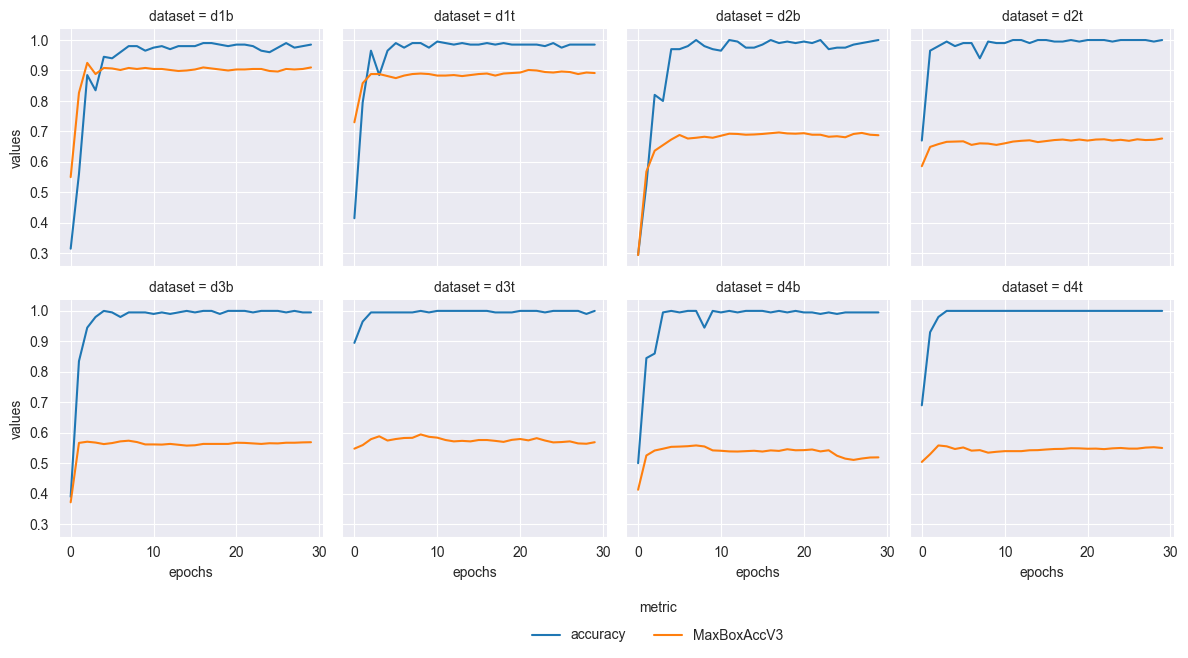
\includegraphics[width=\textwidth]{fig_loc_vs_acc_vgg16_gap_cam_synthetic.png}
    \caption[Training classification versus CAM localization accuracy on VGG16-GAP]{Training classification versus CAM localization accuracy (MaxBoxAccV3 recall) on VGG16-GAP.}
    \caption*{Source: Author}
    \label{fig:loc_vs_acc_vgg16_gap_cam_synthetic}
    \end{center}
\end{figure}

Figure \ref{fig:loc_vs_acc_vgg16_gap_minmaxcam_synthetic} shows training classification and CAM MaxBoxAccV3 recall for model fine-tuned with MinMaxCAM regularization on the different datasets. Here, we observe that models trained for the t-variant datasets show a curve with decreasing MaxBoxAccV3 recall at later training epochs. This is in line with results in Table \ref{tab:maxboxaccv3_recall_vgg16_gap_synthetic}. As Wang \textit{et al.} \cite{wang2021minmaxcam} set out, the condition for common region regularization to work, is that a set of images for the same class should have different backgrounds. This clearly is not the case for the t-variant datasets.

\begin{figure}[ht]
    \begin{center}       
    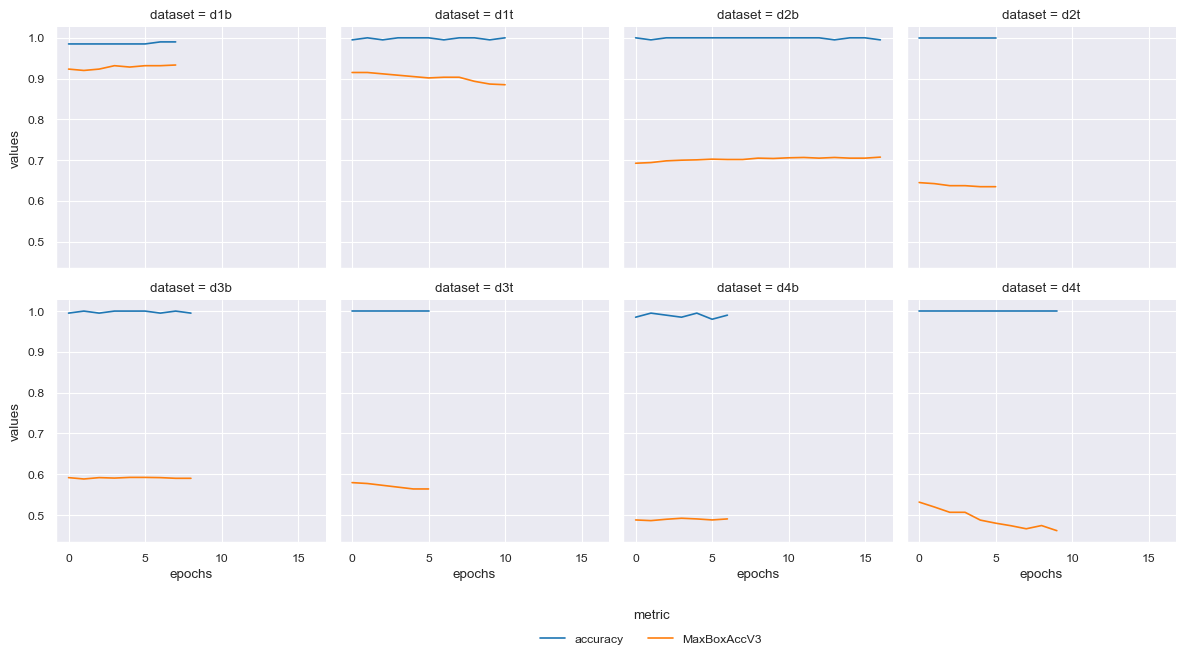
\includegraphics[width=\textwidth]{fig_loc_vs_acc_vgg16_gap_minmaxcam_synthetic.png}
    \caption[Training classification versus localization accuracy for MinMaxCAM on VGG16-GAP]{Training classification versus localization accuracy (MaxBoxAccV3 recall) for MinMaxCAM on VGG16-GAP.}
    \caption*{Source: Author}
    \label{fig:loc_vs_acc_vgg16_gap_minmaxcam_synthetic}
    \end{center}
\end{figure}

\subsubsection{VGG16}
The localization results for VGG16 on the synthetic datasets are shown in Table \ref{tab:maxboxaccv3_recall_vgg16_base_synthetic} for MaxBoxAccV3 recall, in Table \ref{tab:maxboxaccv3_precision_vgg16_base_synthetic} for MaxBoxAccV3 precision, and in Table \ref{tab:pxap_vgg16_base_synthetic} for the PxAP metric. Note that CAM and MinMaxCAM methods cannot be used on VGG16 as this architecture has no \acrshort{gap} layer. Grad-CAM is used here as generalization of CAM.

\begin{table}[ht]
\centering
\begin{tabular}{lrrrrrrrr}
\toprule
 & \multicolumn{8}{c}{VGG16 synthetic (MaxBoxAccV3 recall)} \\
method & d1b & d1t & d2b & d2t & d3b & d3t & d4b & d4t \\
\cmidrule(lr){1-1} \cmidrule(lr){2-9} 
Grad-CAM & \color{teal} \bfseries 81.33 & 68.83 & 51.17 & 46.08 & 46.94 & 45.06 & 45.33 & 44.00 \\
Grad-CAM++ & \color{purple} \bfseries 72.17 & \color{purple} \bfseries 66.83 & \color{purple} \bfseries 37.58 & \color{purple} \bfseries 35.58 & \color{purple} \bfseries 36.33 & \color{purple} \bfseries 31.94 & \color{purple} \bfseries 35.29 & \color{purple} \bfseries 38.75 \\
Score-CAM & 77.50 & \color{teal} \bfseries 69.33 & \color{teal} \bfseries 55.33 & \color{teal} \bfseries 49.42 & \color{teal} \bfseries 50.50 & \color{teal} \bfseries 49.50 & \color{teal} \bfseries 48.08 & \color{teal} \bfseries 46.79 \\
\bottomrule
\end{tabular}
\caption[MaxBoxAccV3 recall for VGG16 on synthetic datasets]{MaxBoxAccV3 recall for VGG16 on synthetic datasets. Column-wise minimum and maximum are highlighted in red and green.}
\label{tab:maxboxaccv3_recall_vgg16_base_synthetic}
\end{table}

\begin{table}[ht]
\centering
\begin{tabular}{lrrrrrrrr}
\toprule
 & \multicolumn{8}{c}{VGG16 synthetic (MaxBoxAccV3 precision)} \\
method & d1b & d1t & d2b & d2t & d3b & d3t & d4b & d4t \\
\cmidrule(lr){1-1} \cmidrule(lr){2-9}
Grad-CAM & 53.29 & 43.62 & 53.78 & 46.13 & 47.38 & 44.70 & 47.99 & 48.13 \\
Grad-CAM++ & \color{purple} \bfseries 29.51 & \color{purple} \bfseries 29.45 & \color{purple} \bfseries 32.24 & \color{purple} \bfseries 29.36 & \color{purple} \bfseries 31.81 & \color{purple} \bfseries 25.84 & \color{purple} \bfseries 31.01 & \color{purple} \bfseries 35.49 \\
Score-CAM & \color{teal} \bfseries 54.05 & \color{teal} \bfseries 47.01 & \color{teal} \bfseries 58.24 & \color{teal} \bfseries 51.22 & \color{teal} \bfseries 52.48 & \color{teal} \bfseries 52.10 & \color{teal} \bfseries 52.36 & \color{teal} \bfseries 53.33 \\
\bottomrule
\end{tabular}
\caption[MaxBoxAccV3 precision for VGG16 on synthetic datasets]{MaxBoxAccV3 precision for VGG16 on synthetic datasets. Column-wise minimum and maximum are highlighted in red and green.}
\label{tab:maxboxaccv3_precision_vgg16_base_synthetic}
\end{table}

\begin{table}[ht]
\centering
\begin{tabular}{lrrrrrrrr}
\toprule
 & \multicolumn{8}{c}{VGG16 synthetic (PxAP)} \\
method & d1b & d1t & d2b & d2t & d3b & d3t & d4b & d4t \\
\cmidrule(lr){1-1} \cmidrule(lr){2-9}
Grad-CAM & \color{teal} \bfseries 69.83 & 59.06 & 57.35 & 45.12 & 51.73 & 52.00 & 56.18 & 54.84 \\
Grad-CAM++ & \color{purple} \bfseries 63.92 & \color{purple} \bfseries 58.11 & \color{purple} \bfseries 42.26 & \color{purple} \bfseries 34.54 & \color{purple} \bfseries 44.73 & \color{purple} \bfseries 38.77 & \color{purple} \bfseries 46.06 & \color{purple} \bfseries 47.34 \\
Score-CAM & 66.44 & \color{teal} \bfseries 60.73 & \color{teal} \bfseries 59.32 & \color{teal} \bfseries 52.59 & \color{teal} \bfseries 58.39 & \color{teal} \bfseries 59.53 & \color{teal} \bfseries 58.25 & \color{teal} \bfseries 58.74 \\
\bottomrule
\end{tabular}
\caption[PxAP for VGG16 on synthetic datasets]{PxAP for VGG16 on synthetic datasets. Column-wise minimum and maximum are highlighted in red and green.}
\label{tab:pxap_vgg16_base_synthetic}
\end{table}

A first observation is that the localization metrics for VGG16 are lower than those for the VGG16-GAP network. An intuitive explanation is that in the VGG16 network there is a less direct relationship between feature activation in the last convolutional layer and the predicted target due to the dense network between the convolutional backbone and the classification output. 

Another important observation is that Score-CAM is the best performing localization method, followed by Grad-CAM. and then by Grad-CAM++ by quite a large margin. The difference between Grad-CAM and Grad-CAM localization results for the VGG16 network seems counter-intuitive with findings of Chattopadhay \textit{et al.} \cite{chattopadhay2018grad}, that Grad-CAM++ is better at explaining multiple object instances than Grad-CAM. A possible indication could be that for the synthetic datasets, Grad-CAM++ seems to activate on larger areas, as illustrated in Fig. \ref{fig:vgg16_base_explanation}.

\begin{figure}[ht]
    \begin{center}
    \begin{subfigure}[b]{\textwidth}
         \centering
         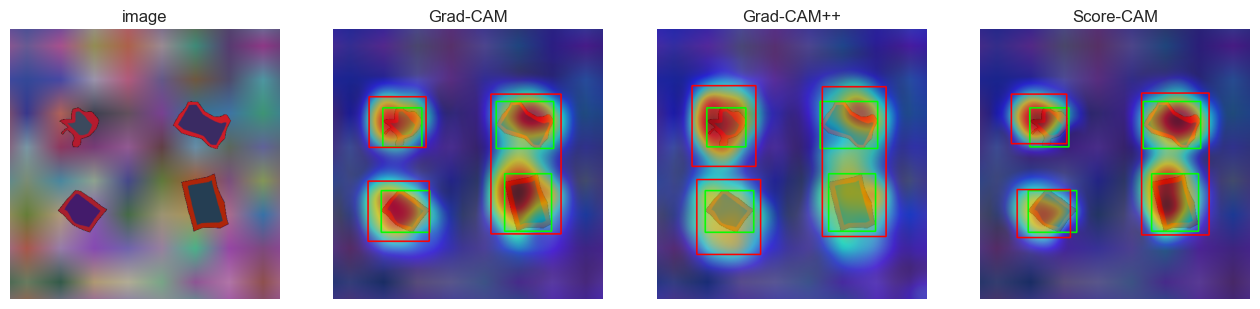
\includegraphics[width=\textwidth]{fig_vgg16_base_d4b.png}
         \caption{Explanation example from d4b dataset.}
         \label{fig:vgg16_base_explanation_d4b}
    \end{subfigure}
    \begin{subfigure}[b]{\textwidth}
         \centering
         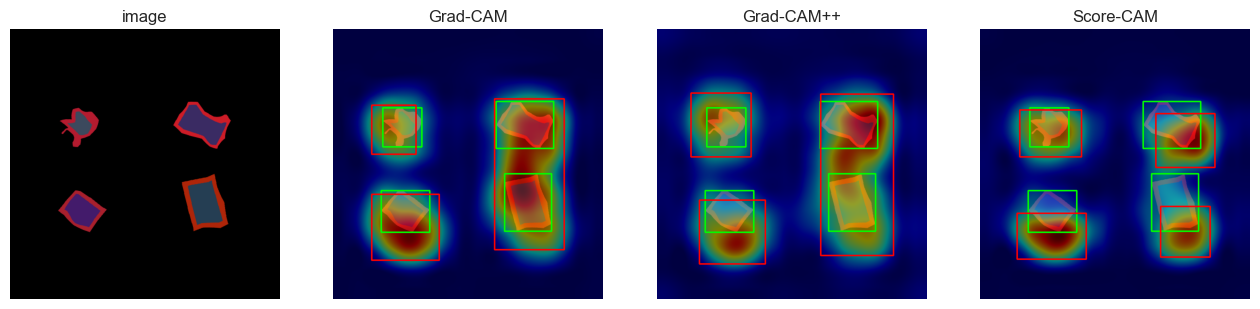
\includegraphics[width=\textwidth]{fig_vgg16_base_d4t.png}
         \caption{Explanation example from d4t dataset.}
         \label{fig:vgg16_base_explanation_d4t}
    \end{subfigure}
    \caption[Explanation maps for localization methods on VGG16 network]{Explanation maps for localization methods on VGG16 network. Heat maps show the activated image areas for the ground truth class. Annotations are given for ground truth (green) and predicted (red) bounding boxes.}
    \caption*{Source: Author}
    \label{fig:vgg16_base_explanation}
    \end{center}
\end{figure}

Finally, we see a similar trend in pair-wise discrepancies between b-variant and t-variant datasets having the same number of object instances as observed for the VGG16-GAP network.  

\subsubsection{ResNet-50}
Localization performance results for the ResNet-50 network on the synthetic dataset are illustrated in Table \ref{tab:maxboxaccv3_recall_resnet50_synthetic} for MaxBoxAccV3 recall, in Table \ref{tab:maxboxaccv3_precision_resnet50_synthetic} for MaxBoxAccV3 precision and in Table \ref{tab:pxap_resnet50_synthetic} for PxAP. Here Grad-CAM is not evaluated as it is identical to CAM for architectures with a \acrshort{gap} architecture.

\begin{table}[ht]
\centering
\begin{tabular}{lrrrrrrrr}
\toprule
 & \multicolumn{8}{c}{ResNet-50 synthetic (MaxBoxAccV3 recall)} \\
method & d1b & d1t & d2b & d2t & d3b & d3t & d4b & d4t \\
\cmidrule(lr){1-1} \cmidrule(lr){2-9}
CAM & \color{purple} \bfseries 84.00 & \color{purple} \bfseries 74.67 & \color{purple} \bfseries 67.08 & \color{purple} \bfseries 71.08 & \color{purple} \bfseries 62.89 & \color{purple} \bfseries 62.61 & \color{purple} \bfseries 59.29 & \color{purple} \bfseries 58.71 \\
Grad-CAM++ & 85.33 & 75.67 & \color{teal} \bfseries \underline{69.33} & 72.08 & \color{teal} \bfseries \underline{66.06} & 65.00 & \color{teal} \bfseries \underline{61.79} & \color{teal} \bfseries \underline{61.13} \\
Score-CAM & \color{teal} \bfseries \underline{85.50} & \color{teal} \bfseries \underline{77.00} & 68.92 & \color{teal} \bfseries 73.58 & 64.89 & \color{teal} \bfseries 65.50 & 61.63 & 60.58 \\
\cmidrule(lr){1-1} \cmidrule(lr){2-9}
MinMaxCAM & 80.33 & \color{purple} \bfseries \underline{68.17} & \color{purple} \bfseries \underline{59.17} & \color{purple} \bfseries \underline{59.08} & \color{purple} \bfseries \underline{56.50} & \color{purple} \bfseries \underline{56.11} & \color{purple} \bfseries \underline{55.92} & \color{purple} \bfseries \underline{52.87} \\
Grad-CAM++ & \color{teal} \bfseries 80.83 & 69.17 & \color{teal} \bfseries 63.83 & 61.92 & \color{teal} \bfseries 61.00 & \color{teal} \bfseries 59.94 & \color{teal} \bfseries 58.96 & \color{teal} \bfseries 57.08 \\
Score-CAM & \color{purple} \bfseries \underline{79.00} & \color{teal} \bfseries 71.17 & 61.00 & \color{teal} \bfseries 62.50 & 58.44 & 59.11 & 58.71 & 56.83 \\
\bottomrule
\end{tabular}
\caption[MaxBoxAccV3 recall for ResNet-50 on synthetic datasets]{MaxBoxAccV3 recall for ResNet-50 on synthetic datasets. First 3 rows are results for model trained without regularization. Last 3 rows show results for model trained with MinMaxCAM regularization. Column-wise minimum and maximum per sub-table are highlighted in red and green. Global column-wise minimum and maximum are underlined.}
\label{tab:maxboxaccv3_recall_resnet50_synthetic}
\end{table}

\begin{table}[ht]
\centering
\begin{tabular}{lrrrrrrrr}
\toprule
 & \multicolumn{8}{c}{ResNet-50 synthetic (MaxBoxAccV3 precision)} \\
method & d1b & d1t & d2b & d2t & d3b & d3t & d4b & d4t \\
\cmidrule(lr){1-1} \cmidrule(lr){2-9}
CAM & \color{purple} \bfseries 75.30 & \color{purple} \bfseries 59.95 & \color{purple} \bfseries 69.48 & \color{purple} \bfseries 73.63 & \color{purple} \bfseries 68.29 & \color{purple} \bfseries 66.17 & \color{purple} \bfseries 65.83 & \color{purple} \bfseries 65.50 \\
Grad-CAM++ & 76.75 & 61.45 & \color{teal} \bfseries \underline{70.99} & 73.84 & \color{teal} \bfseries \underline{70.14} & 67.96 & 66.94 & \color{teal} \bfseries \underline{66.57} \\
Score-CAM & \color{teal} \bfseries \underline{77.58} & \color{teal} \bfseries \underline{64.77} & 69.51 & \color{teal} \bfseries \underline{74.60} & 69.25 & \color{teal} \bfseries \underline{68.70} & \color{teal} \bfseries \underline{67.75} & 65.82 \\
\cmidrule(lr){1-1} \cmidrule(lr){2-9}
MinMaxCAM & 70.21 & \color{purple} \bfseries \underline{49.82} & \color{purple} \bfseries \underline{61.23} & \color{purple} \bfseries \underline{60.03} & \color{purple} \bfseries \underline{61.27} & \color{purple} \bfseries \underline{59.88} & \color{purple} \bfseries \underline{62.59} & \color{purple} \bfseries \underline{58.82} \\
Grad-CAM++ & \color{teal} \bfseries 71.31 & 53.73 & \color{teal} \bfseries 64.93 & \color{teal} \bfseries 62.81 & \color{teal} \bfseries 63.74 & \color{teal} \bfseries 62.68 & \color{teal} \bfseries 63.85 & \color{teal} \bfseries 61.90 \\
Score-CAM & \color{purple} \bfseries \underline{68.87} & \color{teal} \bfseries 55.41 & 61.61 & 62.07 & 62.13 & 62.09 & 63.64 & 61.30 \\
\bottomrule
\end{tabular}
\caption[MaxBoxAccV3 precision for ResNet-50 on synthetic datasets]{MaxBoxAccV3 precision for ResNet-50 on synthetic datasets. First 3 rows are results for model trained without regularization. Last 3 rows show results for model trained with MinMaxCAM regularization. Column-wise minimum and maximum per sub-table are highlighted in red and green. Global column-wise minimum and maximum are underlined.}
\label{tab:maxboxaccv3_precision_resnet50_synthetic}
\end{table}

\begin{table}[ht]
\centering
\begin{tabular}{lrrrrrrrr}
\toprule
 & \multicolumn{8}{c}{ResNet-50 synthetic (PxAP)} \\
method & d1b & d1t & d2b & d2t & d3b & d3t & d4b & d4t \\
\cmidrule(lr){1-1} \cmidrule(lr){2-9} 
CAM & \color{purple} \bfseries 76.85 & \color{purple} \bfseries 65.98 & \color{purple} \bfseries 75.60 & \color{purple} \bfseries 77.27 & 75.32 & \color{purple} \bfseries 73.97 & 74.00 & \color{purple} \bfseries 71.46 \\
Grad-CAM++ & \color{teal} \bfseries 78.02 & 68.86 & \color{teal} \bfseries 76.97 & 78.03 & \color{teal} \bfseries 76.93 & 74.69 & \color{teal} \bfseries 75.31 & 72.10 \\
Score-CAM & 77.97 & \color{teal} \bfseries 69.36 & 76.09 & \color{teal} \bfseries 79.37 & \color{purple} \bfseries 74.63 & \color{teal} \bfseries 75.58 & \color{purple} \bfseries 72.83 & \color{teal} \bfseries 72.92 \\
\cmidrule(lr){1-1} \cmidrule(lr){2-9} 
MinMaxCAM & \color{purple} \bfseries 71.11 & \color{purple} \bfseries 56.26 & \color{purple} \bfseries 63.38 & \color{purple} \bfseries 66.11 & 67.64 & \color{purple} \bfseries 66.99 & \color{purple} \bfseries 68.71 & \color{purple} \bfseries 64.74 \\
Grad-CAM++ & \color{teal} \bfseries 72.56 & 59.92 & \color{teal} \bfseries 66.74 & 68.09 & \color{teal} \bfseries 70.15 & \color{teal} \bfseries 69.25 & \color{teal} \bfseries 70.83 & 66.89 \\
Score-CAM & 71.43 & \color{teal} \bfseries 61.04 & 65.57 & \color{teal} \bfseries 68.20 & \color{purple} \bfseries 67.23 & 68.20 & 69.15 & \color{teal} \bfseries 67.20 \\
\bottomrule
\end{tabular}
\caption[PxAP for ResNet-50 on synthetic datasets]{PxAP for ResNet-50 on synthetic datasets. First 3 rows are results for model trained without regularization. Last 3 rows show results for model trained with MinMaxCAM regularization. Column-wise minimum and maximum per sub-table are highlighted in red and green. Global column-wise minimum and maximum are underlined.}
\label{tab:pxap_resnet50_synthetic}
\end{table}

A similar trend as for VGG16-GAP and VGG16 networks can be observed: Localization performance decreases for increasing number of object instances in images. 

Grad-CAM++ and Score-CAM localization methods perform better than CAM, both for the non-regularized model and for the MinMaxCAM-regularized model. Chattopadhay \textit{et al.} \cite{chattopadhyay2017grad} visually illustrated how taking a weighted combination of positive partial derivatives instead of a global average solves the problem of identifying multiple occurrences of the same class in an image and improper object localization. We quantitatively show that this statement holds for most synthetic datasets on the ResNet-50 network.

The MinMaxCAM-regularized model has lower localization performance than the non-regularized one for the ResNet-50 network. There is room for improvement as we haven't optimized the hyper parameters for MinMaxCAM. Still, it can be observed that both Grad-CAM++ and Score-CAM both improve on the CAM localization results.

\subsection{ImageNet dataset}
In this section we evaluate the localization methods on the ImageNet validation dataset. Multi-instance localization metrics MaxBoxAccV3 recall and precision are used as in previous sections. In addition we illustrate the MaxBoxAcc and MaxBoxAccV2 metrics to benchmark our trained models with results provided by Choe \textit{et al.} \cite{choe2020evaluating} where appropriate. \acrfull{pxap} cannot be used as localization metric as the ImageNet dataset has no ground truth segmentation masks. In following sections, results for VGG16-GAP and ResNet-50 architectures are discussed.

\subsubsection{VGG16-GAP}
We modified a pre-trained VGG16 network into the VGG16-GAP network by replacing the dense network of VGG16 with a \acrshort{gap} layer followed by a single fully connected layer. This newly constructed network is fine-tuned until the loss of the validation dataset hasn't decreased for five consecutive training epochs. The localization results of VGG16-GAP on the ImageNet validation dataset are illustrated in Table \ref{tab:metrics_vgg16_gap_imagenet}.

\begin{table}[ht]
\centering
\begin{tabular}{lrrrr}
\toprule
 & & & \multicolumn{2}{c}{MaxBoxAccV3} \\
method & MaxBoxAcc & MaxBoxAccV2 & precision & recall \\
\cmidrule(lr){1-1} \cmidrule(lr){2-5}
CAM & 61.19 & 60.22 & \color{purple} \bfseries 36.73 & 38.44 \\
Grad-CAM++ & \color{teal} \bfseries 61.29 & \color{teal} \bfseries 60.43 & 36.87 & \color{teal} \bfseries 38.66 \\
Score-CAM & \color{purple} \bfseries 58.44 & \color{purple} \bfseries 57.56 & \color{teal} \bfseries 37.33 & \color{purple} \bfseries 36.48 \\
\bottomrule
\end{tabular}
\caption[Localization metrics for VGG16-GAP on ImageNet]{Localization metrics for VGG16-GAP on ImageNet. Column-wise minimum and maximum are highlighted in red and green.}
\label{tab:metrics_vgg16_gap_imagenet}
\end{table}

The values for the metrics MaxBoxAcc ($61.19$) and MaxBoxAccV2 ($60.22$) for the \acrshort{cam} method closely match the results reported by Choe \textit{et al.} \cite{choe2020evaluating}. Our VGG16-GAP model is thus able to reproduce the results in the \acrshort{wsol} evaluation paper.

MaxBoxAccV3 recall for Score-CAM is 2 percentage points lower than CAM and Grad-CAM++. An intuitive explanation for lower Score-CAM score could be that Score-CAM tends to generate more focused score maps than Grad-CAM++, resulting in less accurate bounding box estimations. 

Due to time constraints, we haven't trained a MinMaxCAM-regularized model for the VGG16-GAP network on ImageNet.

\subsubsection{ResNet-50}

For the ResNet-50 network we evaluate four different localization methods on the ImageNet validation dataset. The results of these experiments are illustrated in Table \ref{tab:metrics_resnet50_imagenet}. The MaxBoxAcc and MaxBoxAccV2 metrics for the CAM method have lower scores than those reported by Choe \textit{et al.} (57.60 and 57.25 versus 64.2 and 63.7). An explanation for this discrepancy, could be that we used a pre-trained ResNet-50 model where the authors of the mentioned paper did a grid search on hyper parameters to improve localization. 

The MaxBoxAccV3 metric has slightly lower values than those that we reported for the VGG16-GAP network, but the same trend can be observed. Grad-CAM++ is the best performing method and Score-CAM score is nearly two percentage points below the Grad-CAM++ one. MinMaxCAM performs slightly worse than CAM. This is opposite to the results noted by Wang \textit{et al.} \cite{wang2021minmaxcam}, who illustrated that MinMaxCAM improves MaxBoxAcc by 2.5 percentage points compared to CAM. 

We haven't reproduced the results of the authors of the MinMaxCAM paper \cite{wang2021minmaxcam}, due to lack of reference values for the regularization weights. Given the values to reproduce the author's results, the multi-instance localization metric MaxBoxAccV3 could be further improved for MinMaxCAM.

\begin{table}[ht]
\centering
\begin{tabular}{lrrrr}
\toprule
 & & & \multicolumn{2}{c}{MaxBoxAccV3} \\
method & MaxBoxAcc & MaxBoxAccV2 & precision & recall \\
\cmidrule(lr){1-1} \cmidrule(lr){2-5}
CAM & 57.60 & 57.25 & 30.55 & 36.58 \\
Grad-CAM++ & \color{teal} \bfseries 59.40 & \color{teal} \bfseries 58.55 & 31.17 & \color{teal} \bfseries 37.53 \\
MinMaxCAM & 58.81 & 57.26 & \color{teal} \bfseries 43.70 & 36.02 \\
Score-CAM & \color{purple} \bfseries 56.19 & \color{purple} \bfseries 56.35 & \color{purple} \bfseries 29.60 & \color{purple} \bfseries 35.92 \\
\bottomrule
\end{tabular}
\caption[Metrics for ResNet-50 on ImageNet]{Metrics for ResNet-50 on ImageNet.}
\label{tab:metrics_resnet50_imagenet}
\end{table}

%- MaxBoxAcc, PxAP for (vgg16, resnet50), (synthetic, imagenet), CAM methods
%- discuss and explain differences
%- show multiple examples of each method, architecture, dataset
%- discuss and compare results


\section{Computational complexity}
In this section we evaluation the computational complexity of \acrshort{cam} methods used in our experiments. We measure the localization method runtime for ResNet-50 network on the ImageNet validation dataset. The mean runtime and standard deviation per batch of images, and the aggregated runtime for the complete  dataset is computed. The results for each method is illustrated in Table \ref{tab:runtime_resnet50_imagenet}.

\begin{table}[ht]
\centering
\begin{tabular}{lrrrr}
\toprule
\multicolumn{2}{c}{} & \multicolumn{3}{c}{runtime (ms)} \\
method & batch size (bytes) & sum & mean & std \\
\cmidrule(lr){1-2} \cmidrule(lr){3-5}
CAM & 512 & 309209 & 3155 & 225 \\
Grad-CAM++ & 128 & 804349 & 2057 & 140 \\
MinMaxCAM & 512 & 299392 & 3055 & 982 \\
Score-CAM & 512 & \bfseries 97763413 & 997585 & 34463\\
\bottomrule
\end{tabular}
\caption[Method runtime for ResNet-50 on ImageNet validation dataset]{Method runtime for ResNet-50 on ImageNet validation dataset.}
\label{tab:runtime_resnet50_imagenet}
\end{table}

The runtime is measured as the time it takes to compute score maps for the 50000 images in the ImageNet validation dataset. Runtime exludes operations to load and preprocess the images. Grad-CAM was not measured as this method specializes to the CAM method for ResNet-50. However, it has the same order of complexity as Grad-CAM++ due to the equal number of forward and backward passes. Grad-CAM++ takes nearly three times the runtime of the CAM method. This could indicate that backward passes more costly than forward passes.

Each method computes a score map as a weighted combination of feature maps in the final convolutional layer. CAM (MinMaxCAM uses the CAM method for computing score maps), takes as weights the parameters learned in the single fully connected layer, which is a very cheap operation. Grad-CAM and Grad-CAM++ compute weights from the backprogagated gradients in the final convolutional layer. Similarly this operation is not computationally expensive.

The most computationally costly method by far is Score-CAM. This method computes the weights for the feature maps by feeding the network with the product of each feature map with the original image to obtain the classification score after softmax. As ResNet-50 has 2048 channels in its final convolutional layer, this is an expensive operation.

\section{Localization improvements}

Using the iterative localization method proposed in section \ref{sec:method_localization_improvement}, we analyze the effect of this method for VGG16-GAP and ResNet-50 architectures on the synthetic and ImageNet datasets. We use the same models that were trained for the non-iterative approach.

\subsection{Recall versus precision}
The aim of the iterative approach is to maximize the accurate localization of ground truth object instances. This is measured by the recall metric. If we would have a localization method that exhaustively generates bounding boxes of different granularity, then such method would accurately localize most object instances and thus have a high recall. At the same time this method would suffer from a lot of false positives, i.e., many localized objects would not match with the actual ground truth instances. Hence, the precision would be low.

To measure the impact of the iterative localization method we want to measure both precision and recall. Ideally, we would like to have a localization method that has good precision and recall. If we equally care about precision and recall, the f1 score represents the harmonic mean between precision and recall.

\subsection{Evaluation on synthetic datasets}
Here we evaluate the results of the iterative localization method for the VGG16-GAP network and the ResNet-50 network on the synthetic test datasets. We only tests the datasets that have images with a background to evaluate the effect of using different bounding box mask strategies.

\subsubsection{VGG16-GAP}
The combinations of datasets, localization methods, mask strategies, merge strategies and iteration stop criteria is too large to draw conclusions from. Therefore we graphically represent the result as follows:
\begin{itemize}
    \item Per dataset and localization method, we plot a two-dimensional plot with precision and recall axes for the different mask strategies, merge strategies and stop criteria.
    \item The precision and recall for the non-iterative approach is plotted as two orthogonal lines
\end{itemize}

\begin{figure}[ht]
    \begin{center}       
    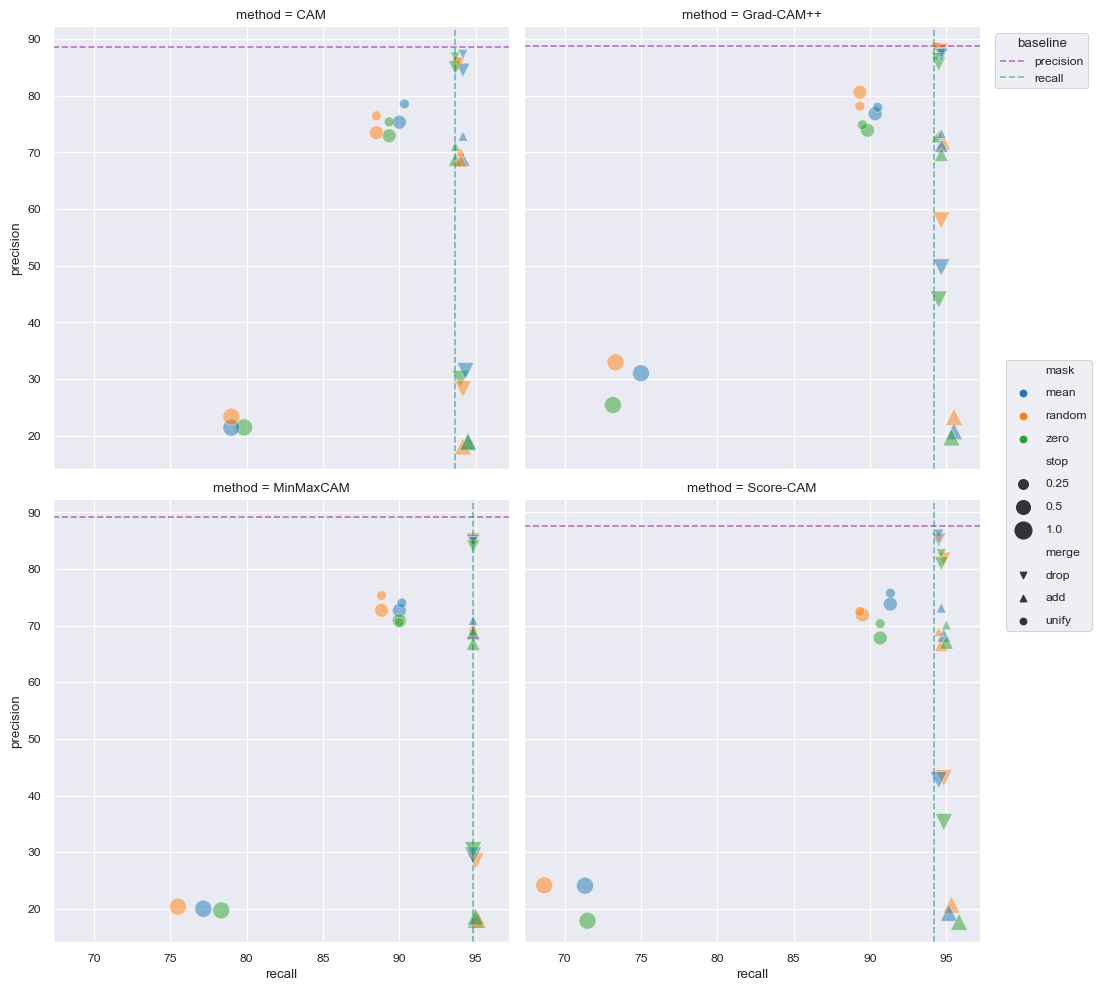
\includegraphics[width=1.0\textwidth]{images/fig_iter_vgg16_gap_syn_d1b.png}
    \caption[Iterative localization performance for VGG16-GAP on synthetic dataset d1b]{Iterative localization performance for VGG16-GAP on synthetic datasets d1b. The cross-hair lines mark the best precision and recall for non-iterative localization.}
    \caption*{Source: Author}
    \label{fig:prec_iter_vgg16_gap_syn_d1b}
    \end{center}
\end{figure}

\begin{figure}[ht]
    \begin{center}       
    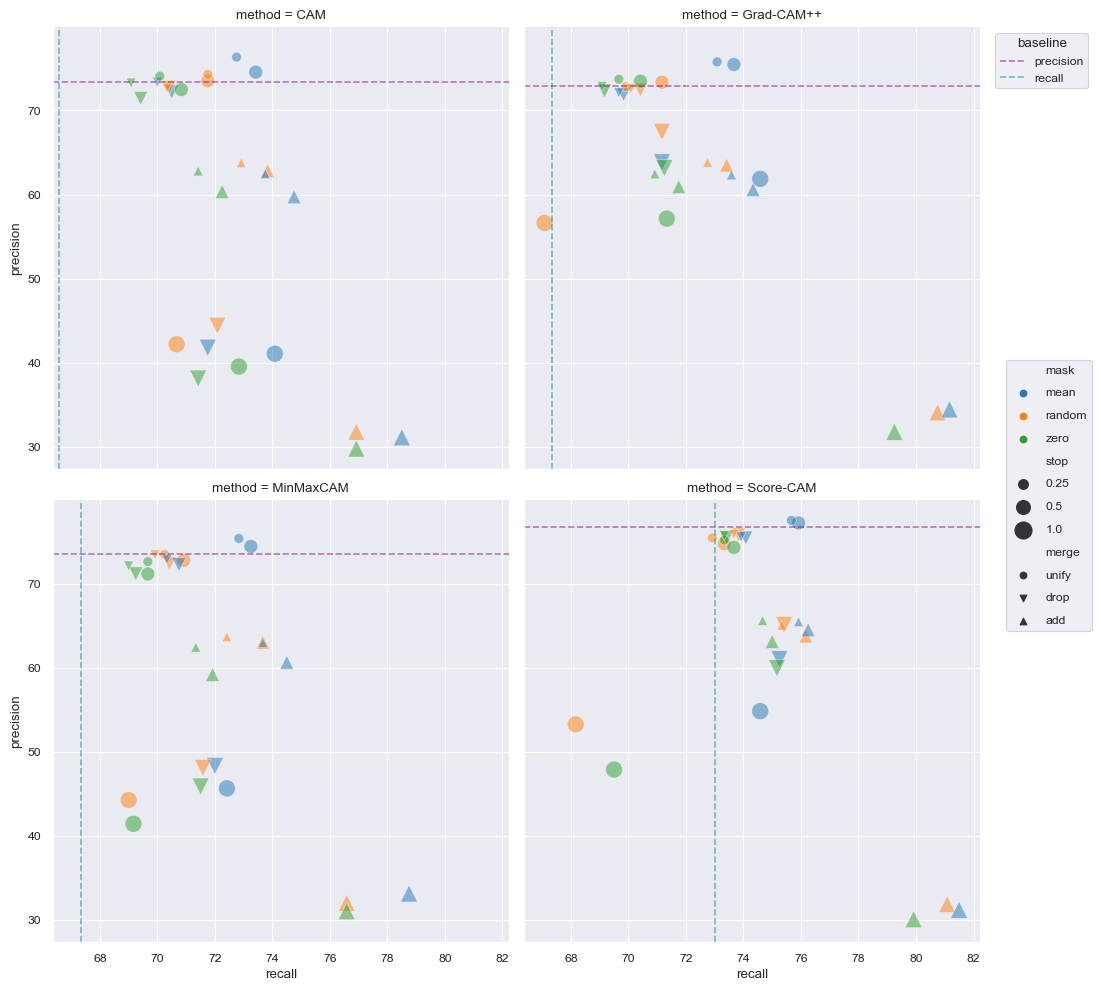
\includegraphics[width=1.0\textwidth]{images/fig_iter_vgg16_gap_syn_d2b.png}
    \caption[Iterative localization performance for VGG16-GAP on synthetic dataset d2b]{Iterative localization performance for VGG16-GAP on synthetic datasets d2b. The cross-hair lines mark the best precision and recall for non-iterative localization.}
    \caption*{Source: Author}
    \label{fig:prec_iter_vgg16_gap_syn_d2b}
    \end{center}
\end{figure}

\begin{figure}[ht]
    \begin{center}       
    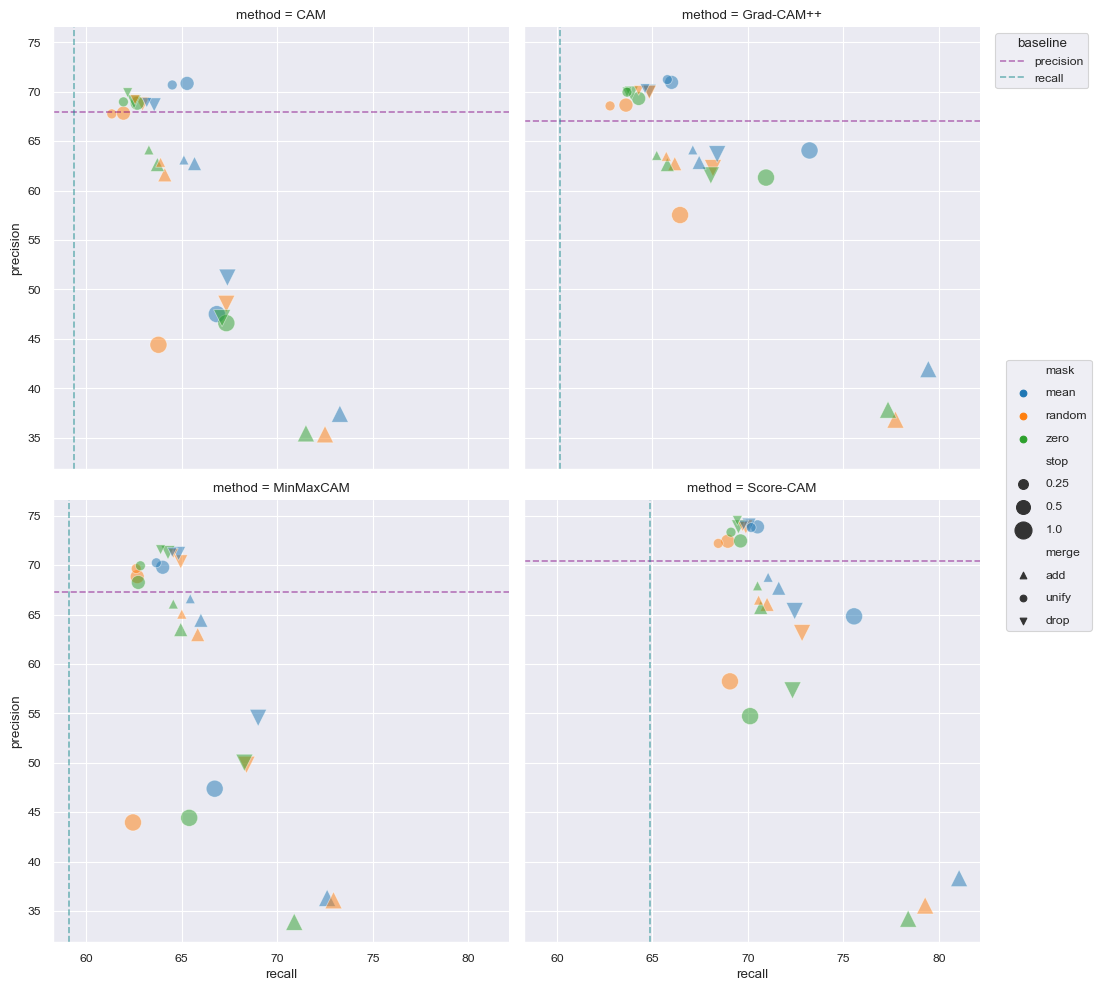
\includegraphics[width=1.0\textwidth]{images/fig_iter_vgg16_gap_syn_d3b.png}
    \caption[Iterative localization performance for VGG16-GAP on synthetic dataset d3b]{Iterative localization performance for VGG16-GAP on synthetic datasets d3b. The cross-hair lines mark the best precision and recall for non-iterative localization.}
    \caption*{Source: Author}
    \label{fig:prec_iter_vgg16_gap_syn_d3b}
    \end{center}
\end{figure}

\begin{figure}[ht]
    \begin{center}       
    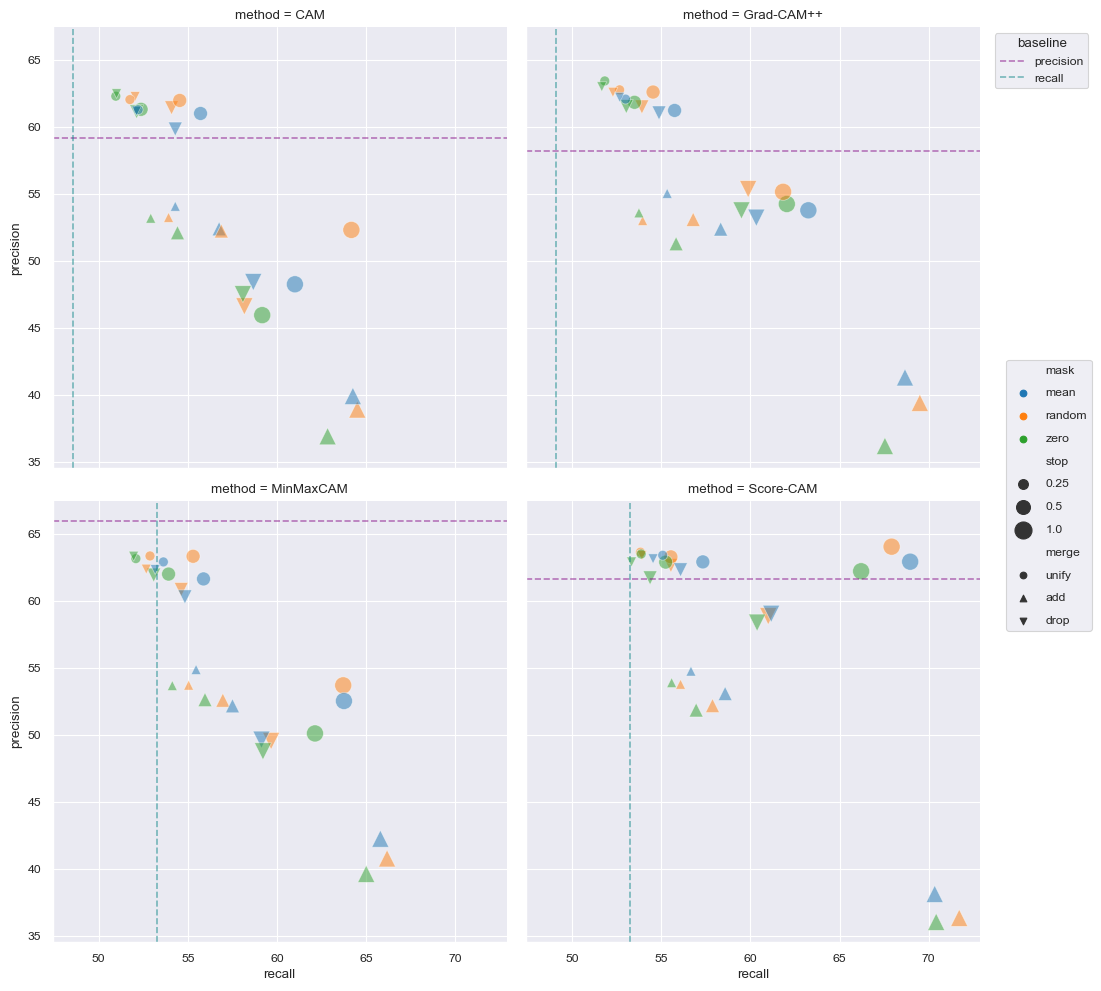
\includegraphics[width=1.0\textwidth]{images/fig_iter_vgg16_gap_syn_d4b.png}
    \caption[Iterative localization performance for VGG16-GAP on synthetic dataset d4b]{Iterative localization performance for VGG16-GAP on synthetic datasets d4b. The cross-hair lines mark the best precision and recall for non-iterative localization.}
    \caption*{Source: Author}
    \label{fig:prec_iter_vgg16_gap_syn_d4b}
    \end{center}
\end{figure}

\subsubsection{ResNet-50}

\subsection{Evaluation for ResNet-50 on ImageNet dataset}

\begin{figure}[ht]
    \begin{center}       
    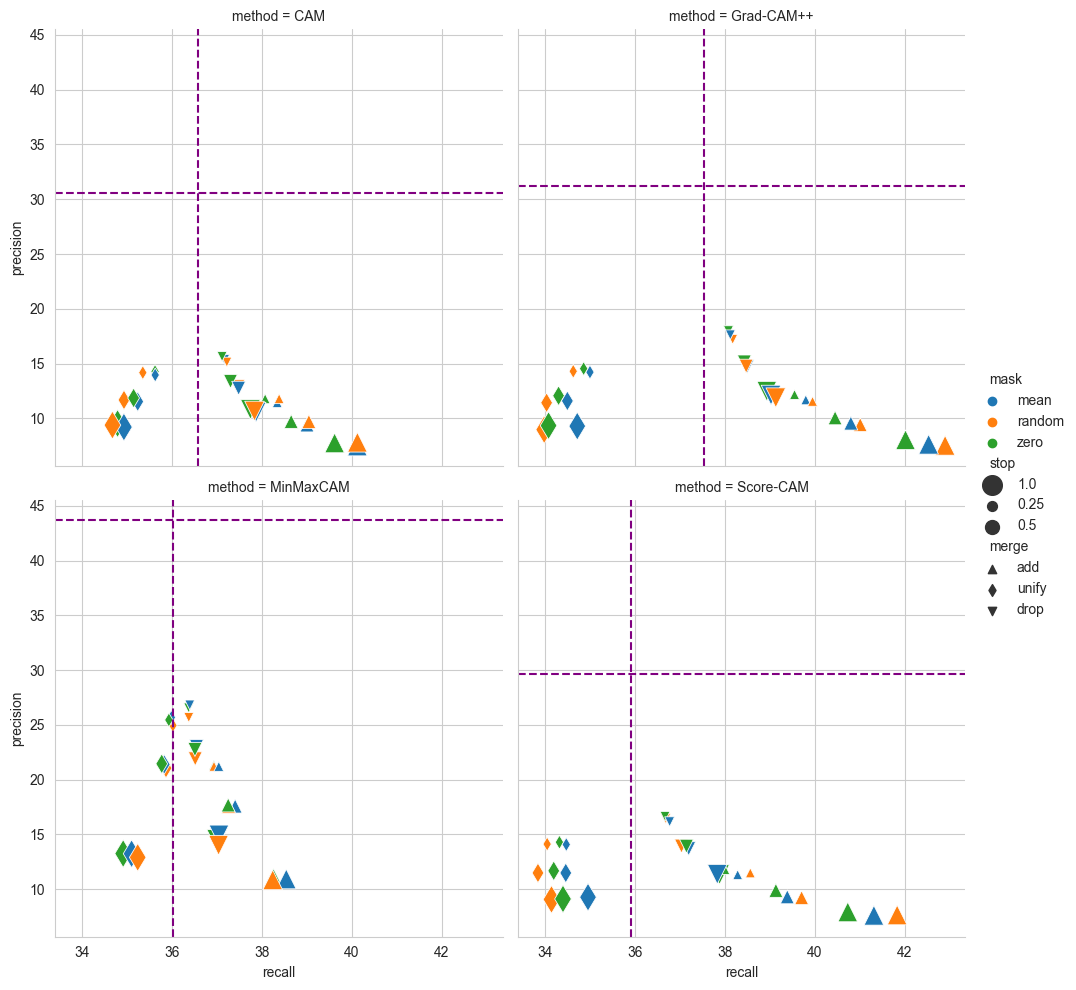
\includegraphics[width=1.0\textwidth]{fig_iter_resnet50_imagenet.png}
    \caption[Iterative localization performance for ResNet-50 on ImageNet dataset]{Iterative localization performance for ResNet-50 on ImageNet dataset. The cross-hair lines mark the best precision and recall for non-iterative localization.}
    \caption*{Source: Author}
    \label{fig:prec_iter_resnet50_imagenet}
    \end{center}
\end{figure}
